\documentclass{standalone}
\usepackage{amsmath}
\usepackage[T1]{fontenc}
\usepackage[utf8]{inputenc}

\usepackage[usenames,dvipsnames]{xcolor}

\usepackage{tikz}
\usetikzlibrary{arrows, shapes, matrix}

\begin{document}

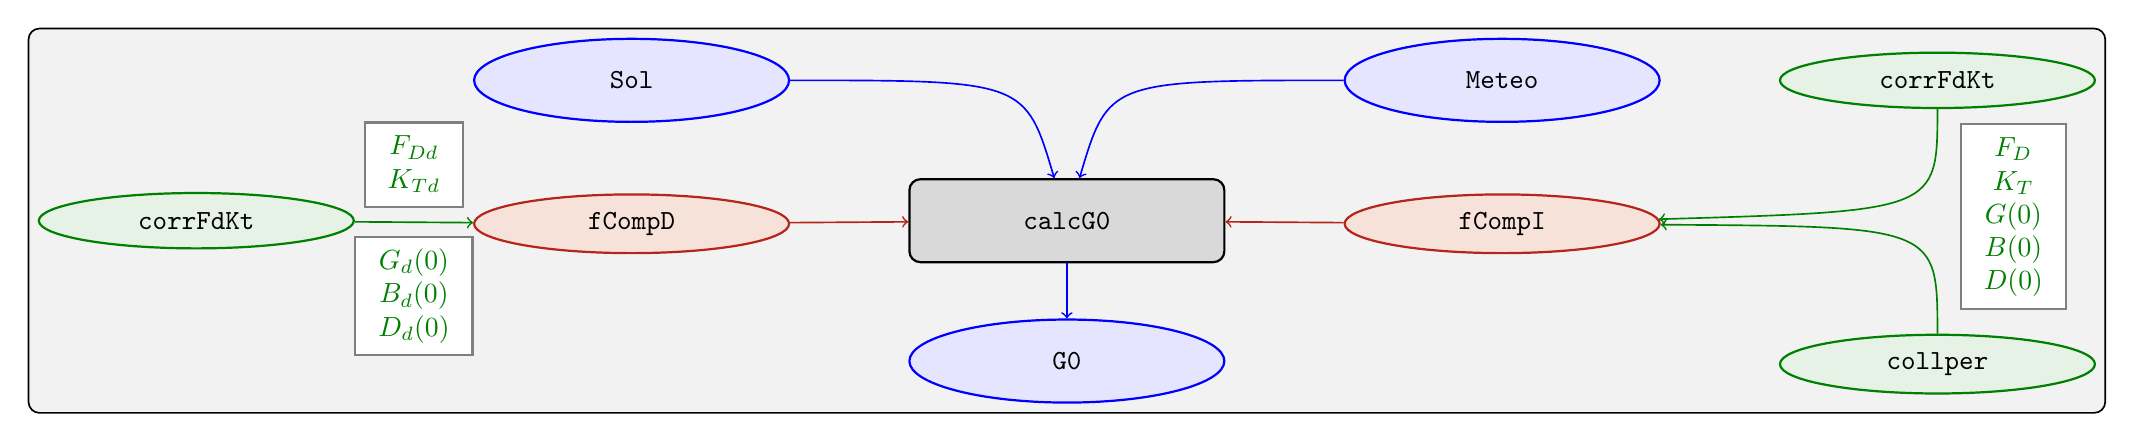
\begin{tikzpicture}[auto,
  method/.style={rectangle, rounded corners, draw=black, thick, fill=gray!30,
    minimum height = 3em, align=flush center, inner sep=1pt},
  %
  function/.style ={draw=BrickRed, thick, ellipse, fill=BrickRed!10,
    minimum height=2em},
  % 
  class/.style ={draw=Blue, thick, ellipse, fill=Blue!10,
    minimum height=3em},
  %
  utils/.style ={draw=Green, thick, ellipse, fill=Green!10,
    minimum height=2em},
  %
  simple/.style ={draw=black!50, thick, rectangle, fill=white}
  ]
  
  \tikzset{every path/.style={line width=.6pt}}

  \begin{scope}
    \matrix [matrix of nodes, rounded corners, fill=gray!10, draw=black, column
  sep=15mm,row sep=7mm, minimum width=4cm] (Geometry) {
    %%%%%%%%%%%%%%%%%%%%%%%%%%%%%%% 
    \node {}; &
    \node [class] (sol) {\texttt{Sol}}; &
    \node {}; &
    \node [class] (meteo) {\texttt{Meteo}}; &
    \node [utils] (corrFdKti) {\texttt{corrFdKt}}; \\
    %%%%%%%%%%%%%%%%%%%%%%%%%%%%%%%
    \node [utils] (corrFdKtd) {\texttt{corrFdKt}}; &
    \node [function] (fCompD) {\texttt{fCompD}}; &
    \node [method] (calcG0) {\texttt{calcG0}}; &
    \node [function] (fCompI) {\texttt{fCompI}}; &
    \node {}; \\
    %%%%%%%%%%%%%%%%%%%%%%%%%%%%%%%
    \node {}; &
    \node {}; &
    \node [class] (G0) {\texttt{G0}}; &
    \node {}; &
    \node [utils] (collper) {\texttt{collper}}; \\
  };
\end{scope}

\begin{scope}
  \draw [->, Blue] (sol) .. controls ++(0:5) .. (calcG0);
  \draw [->, Blue] (meteo) .. controls ++(0:-5) .. (calcG0);
  \draw [->, BrickRed] (fCompD) -- (calcG0);
  \draw [->, BrickRed] (fCompI) -- (calcG0);
  \draw [->, Blue] (calcG0) -- (G0);
  \draw [->, Green] (corrFdKtd) -- (fCompD)
  node [midway, simple, below, yshift=-0.5em] {$
    \begin{array}{c}
      G_d(0)\\
      B_d(0)\\
      D_d(0)\\
    \end{array}
    $}
  node [midway, simple, above, yshift=0.5em] {$
    \begin{array}{c}
      F_{Dd}\\
      K_{Td}\\
    \end{array}
    $};
  \draw [->, Green] (corrFdKti) .. controls ++(-90:1.66) .. (fCompI)
  node [midway, below, simple, yshift=2.75em, xshift=4em] {$
    \begin{array}{c}
      F_D\\
      K_T\\ 
      G(0)\\
      B(0)\\
      D(0)\\
    \end{array}
    $};
  \draw [->, Green] (collper) .. controls ++(90:1.75) .. (fCompI);
\end{scope}
  
\end{tikzpicture}

\end{document}
